\subsection{Įvykių kaupimas}

Šiame skyriuje yra aprašomos žinios apie įvykių kaupimą, pliusus ir minusus, įvykių srautus bei įvykių kaupimą funkciniame programavime remiantis daugiausia Vaughn Vernon surinkta ir aprašyta informacija \cite{vernon2013implementing}.

\subsubsection{Įvadas}

Kartais verslui svarbu fiksuoti objekto pasikeitimus domeno modelyje. Šiuos pasikeitimus galima stebėti skirtingais būdais. Įprastai yra pasirenkama stebėti kai esybė yra:

\begin{itemize}

	\item sukurta,

	\item paskutinį kartą modifikuota

	\item bei kas atliko modifikaciją.

\end{itemize}

Tačiau šis būdas nepateikia jokios informacijos apie vienkartinius pasikeitimus.

Atsiradus poreikiui stebėti pasikeitimus detaliau, verslas reikalauja dar daugiau metaduomenenų, ko pasekoje tokie faktai kaip individualios operacijos laiko tekmėje bei jų įvykdymo laikas tampa svarbūs. Šie poreikiai verčia įvesti audito žurnalą fiksuoti labai tikslias panaudojimo atvejų metrikas, tačiau pastarasis būdas turi apribojimų. Jis gali atskleisti dalį informacijos apie tai kas nutiko sistemoje, leisti rasti bei ištaisyti dalį riktų bei klaidų programinėje įrangoje. Bet audito žurnalas neleidžia patikrinti domeno objekto būsenos prieš ir po tam tikrų pasikeitimų. O jeigu būtų galima išgauti daugiau informacijos iš pasikeitimų stebėjimo?

Visi programinės įrangos kūrėjai susiduria su labai tiksliu pasikeitimų stebėjimu. Įprastas ir populiarus pavyzdys yra išeities kodo saugyklos, tokios kaip CVS\footnote{http://www.nongnu.org/cvs/}, Subversion\footnote{http://subversion.apache.org/}, Git\footnote{http://git-scm.com/} arba Mercurial\footnote{http://mercurial.selenic.com/}. Visos šios pataisų valdymo sistemos leidžia stebėti pirminių failų pasikeitimus. Įrankiai leidžia peržiūrėti išeities kodo artefaktus nuo pačios pirmosios pataisos iki paskutinės. Kai visi išeities failai yra nusiunčiami į pataisų kontrolės sistemą, ši gali stebėti pasikeitimus viso programinės įrangos kūrimo gyvavimo ciklo metu.

Jeigu šis principas būtų pritaikytas vienai esybei, tada vienam agregatui\footnote{http://martinfowler.com/bliki/DDD\_Aggregate.html} bei galiausiai kiekvienam modelio agregatui, galima suprasti kokią naudą atneša sistemos objektų pasikeitimų stebėjimas:

\begin{itemize}

	\item Kas būtent nutiko modelyje, jog agregato egzempliorius buvo sukurtas?

	\item Kas nutiko agregato egzemplioriui bėgant laikui? (Operacijų požiūriu)

\end{itemize}

Turint visų atliktų operacijų istoriją, galima palaikyti laikinus modelius. Toks kaitos stebėjimas yra įvykių kaupimo principas. \ref{pic:es} diagramoje pateikta šio principo aukšto lygio reprezentacija. Agregatai publikuoja įvykius, kurie yra išsaugomi įvykių saugykloje ir naudojami sekti modelio būsenos pasikeitimus. Verta paminėti, jog įvykiai reprezentuoja tam tikrą būsenos pasikeitimą bėgant laikui, todėl jie nėra atnaujinami arba ištrinami. Saugykla nuskaito įvykius iš įvykių saugyklos ir pritaiko juos vieną po kito taip atkurdama agregato būseną. 

\begin{figure}[ht]
	\centering
	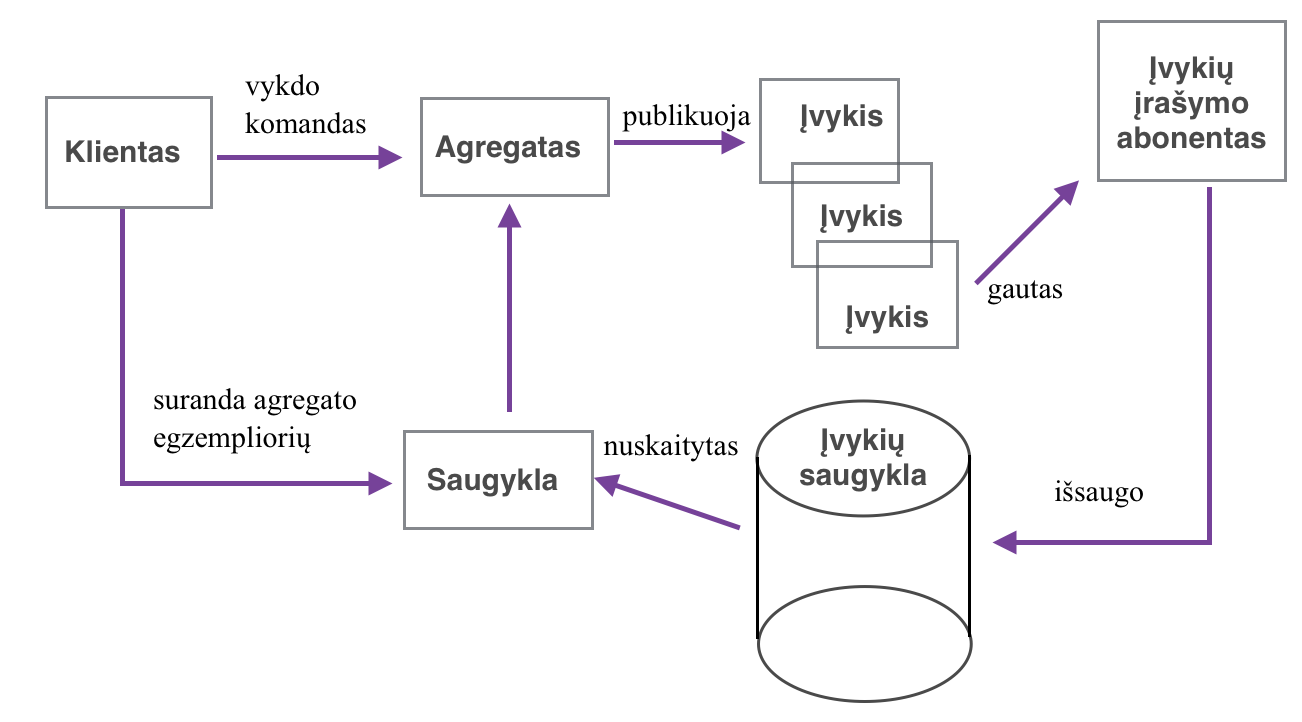
\includegraphics[width=0.9\linewidth]{pics/es.png}
	\caption{Įvykių kaupimo aukšo lygio reprezentacija}
	\label{pic:es}
\end{figure}

\subsubsection{Įvykių kaupimo privalumai ir trūkumai}

Kaip saugojimo mechanizmas, įvykių kaupimas stipriai skiriasi ir pakeičia ORM\footnote{http://www.orm.net/} įrankį. Kadangi įvykiai dažnai įrašomi kaip dvejetainės reprezentacijos, jie negali būti optimaliai naudojami užklausoms atlikti. Faktiškai įvykių kaupimu pagrįstoms saugykloms tereikia vienos operacijos - gauti įrašus pagal unikalią agregato tapatybę \cite{CQRS:GregYoung}. To pasekoje užklausom daryti reikia kito kelio. Dažniausiai tam pasirenkamas CQRS\footnote{http://martinfowler.com/bliki/CQRS.html} principas \cite{Betts:2013:ECE:2509680}. 

Įvykių istorija gali padėti surasti bei ištaisyti sistemos defektus bei klaidas \cite{SeanFitz2012}. Derinimas naudojant istoriją visų veiksmų, kurie nutiko sistemoje, turi didžiulį pranašumą. Įvykių kaupimas gali vesti prie didelio našumo domeno modelių, tai yra palaikyti ypač didelį skaičių operacijų per sekundę. Pavyzdžiui, įrašymas į vieną duomenų saugyklos lentelę yra ypač greitas. Negana to, tai leidžia CQRS užklausų modelį išplėsti horizontaliai, nes duomenų šaltinio atnaujinimai įvykdomi fone, kai įvykių saugykla yra atnaujinama naujais įvykiais.

\subsubsection{Įvykių kaupimas funkciniame programavime}

Vaughn Vernon pateikia keletą pastebėjimų apie įvykių kaupimą funkciniame programavime, kurie gali būti naudingi atliekant projektinius sprendimus bei eksperimentinį tyrimą:

\begin{itemize}

	\item Agregatas projektuojamas kaip nekintantis būsenos įrašas kartu su funkcijomis, kurios keičia būseną. Šios funkcijos paprasčiausiai priima būsenos įrašą ir įvykių argumentus ir gražina naują būsenos įrašą kaip rezultatą. Tokia funkcija pavaizduota \ref{aggregate} kodo pavyzdyje.

\begin{lstlisting}[caption=- agregato būsenos keitimas, label=aggregate]

	Funkcija<Busena, Ivykis, Busena>

\end{lstlisting}

	\item Dabartinė agregato būsena gali būti apibrėžta kaip suskleidimas į kairę visų praeities įvykių, kurie yra perduodami būseną keičiančiai funkcijai.

	\item Agregato metodai gali būti išreikšti kaip kolekcija funkcijų be būsenos.

	\item Įvykių saugykla gali būti suvokiama bei naudojama kaip funkcinė duomenų bazė, nes ji perduoda argumentus funkcijoms, kurios keičia agregato būseną.

\end{itemize}

\subsection{Išvados}

Literatūros analizės metu remiantis kitų autorių patirtimi:

\begin{itemize}

\item išnagrinėtas funkcinis-reaktyvus programavimas,

\item išnagrinėtas įvykių kaupimo principas,

\item išnagrinėti įvykių srautai bei operacijos su jais,

\item susipažinta su įvykių kaupimu funkciniame programavime,

\item įvaldyta sąvokų sistema, susijusi su nagrinėjama tematika.

\end{itemize}